\section{晶体光学}
\subsection{双各向异性介质}

在线性介质中，电磁场的本构关系总能写作
\begin{equation*}
	\vb{D} = \vb{\varepsilon} \cdot \vb{E} + \vb{\xi} \cdot \vb{H}, \quad
	\vb{B} = \vb{\zeta} \cdot \vb{E} + \vb{\mu} \cdot \vb{H}.
\end{equation*}

当 \(\vb{\xi},\ \vb{\zeta}\) 非零时，称为双各向异性（或双各向同性）介质.当 \(\vb{\xi},\ \vb{\zeta}\) 均为零时，称为各向异性（或双各向同性）介质.先考虑双各向异性介质.

注意到 \(\vb{E},\ \vb{D}\) 关于时间反演不变、\(\vb{H},\ \vb{B}\) 关于时间反演反号，根据 Onsager 关系，当介质存在偏置电磁场 \((\vb{D}_0, \vb{H}_0)\) 时，线性系数应当满足
\begin{equation*}
	\vb{\varepsilon}(\vb{D}_0, \vb{H}_0) = \vb{\varepsilon}^\mathrm{T}(\vb{D}_0, -\vb{H}_0),\quad
	\vb{\mu}(\vb{D}_0, \vb{H}_0) = \vb{\mu}^\mathrm{T}(\vb{D}_0, -\vb{H}_0),\quad
	\vb{\xi}(\vb{D}_0, \vb{H}_0) = -\vb{\zeta}^\mathrm{T}(\vb{D}_0, -\vb{H}_0).
\end{equation*}

大多数情况下不考虑偏置，即线性系数总是满足
\begin{equation*}
	\vb{\varepsilon} = \vb{\varepsilon}^\mathrm{T}, \quad
	\vb{\mu} = \vb{\mu}^\mathrm{T}, \quad
	\vb{\xi} = -\vb{\zeta}^\mathrm{T}.
\end{equation*}

特别地，若介质不存在损耗，也即能量守恒方程
\begin{equation*}
	\oint_{\partial V} \frac{1}{2}\Re (\vb{E}\times\vb{H}^*)\cdot\d \vb{S} = -\int_V \frac{1}{2}\Re(\vb{E}\cdot\vb{J}^*)\d V - \omega\int_V \frac{1}{2}\Im (\vb{H}^*\cdot\vb{B} - \vb{E}\cdot\vb{D}^*)\d V.
\end{equation*}
之中，介质损耗功率体密度为零
\begin{equation*}
	p_{\text{abs}} = \frac{\omega}{2}\Im\!\left(\vb{H}^*\cdot\vb{B} - \vb{E}\cdot\vb{D}^*\right) = \frac{\omega}{4i}\begin{pmatrix}\vb{E}^\dagger,\, \vb{H}^\dagger\end{pmatrix}\cdot\begin{pmatrix}\vb{\varepsilon}^\dagger - \vb{\varepsilon} & \vb{\zeta}^\dagger - \vb{\xi} \\ \vb{\xi}^\dagger - \vb{\zeta} & \vb{\mu}^\dagger - \vb{\mu}\end{pmatrix}\cdot\begin{pmatrix}\vb{E} \\ \vb{H}\end{pmatrix} = 0.
\end{equation*}
得到，无论是否存在偏置，总有
\begin{equation*}
	\vb{\varepsilon}^\dagger = \vb{\varepsilon}, \quad
	\vb{\mu}^\dagger = \vb{\mu}, \quad
	\vb{\xi} = \vb{\zeta}^\dagger.
\end{equation*}

这说明，对于无偏置无损耗的线性介质，\(\vb{\varepsilon},\ \vb{\mu}\) 必然是实对称矩阵，\(\vb{\xi},\ \vb{\zeta}\) 的矩阵元必然全部是虚数且 \(\vb{\xi} = -\vb{\zeta}^\mathrm{T}\).

将本构关系代入麦克斯韦方程组
\begin{equation*}
	\nabla\cdot\vb{D}=0,\quad \nabla\cdot\vb{B}=0,\quad \nabla\times\vb{E}=-\frac{\partial\vb{B}}{\partial t},\quad \nabla\times\vb{H}=\frac{\partial\vb{D}}{\partial t}.
\end{equation*}
得到
\begin{equation*}
	&\frac{\partial\vb{E}}{\partial t} = \vb{\varepsilon}^{-1}\cdot\left(\nabla\times\vb{H} - \vb{\xi}\cdot\frac{\partial\vb{H}}{\partial t}\right),\quad
	\frac{\partial\vb{H}}{\partial t} = -\vb{\mu}^{-1}\cdot\left(\nabla\times\vb{E} + \vb{\zeta}\cdot\frac{\partial\vb{E}}{\partial t}\right)\\
	&\nabla\times\left(\vb{\mu}^{-1}\cdot\left(\nabla\times\vb{E}\right)\right) + \left(\vb{\varepsilon} - \vb{\xi}\cdot\vb{\mu}^{-1}\cdot\vb{\zeta}\right)\cdot\frac{\partial^2\vb{E}}{\partial t^2} = -\nabla\times\left(\vb{\mu}^{-1}\cdot\vb{\zeta}\cdot\frac{\partial\vb{E}}{\partial t}\right) + \vb{\xi}\cdot\vb{\mu}^{-1}\cdot\left(\nabla\times\frac{\partial\vb{E}}{\partial t}\right)\\
	&\nabla\times\left(\vb{\varepsilon}^{-1}\cdot\left(\nabla\times\vb{H}\right)\right) + \left(\vb{\mu} - \vb{\zeta}\cdot\vb{\varepsilon}^{-1}\cdot\vb{\xi}\right)\cdot\frac{\partial^2\vb{H}}{\partial t^2} = \nabla\times\left(\vb{\varepsilon}^{-1}\cdot\vb{\xi}\cdot\frac{\partial\vb{H}}{\partial t}\right) - \vb{\zeta}\cdot\vb{\varepsilon}^{-1}\cdot\left(\nabla\times\frac{\partial\vb{H}}{\partial t}\right).
\end{equation*}

下面以此为基础，考虑介质中电磁波的传播.假设介质均匀，对于波动因子为 \(e^{i\left(\vb{k}\cdot\vb{r}-\omega t\right)}\) 的平面波，方程化简为
\begin{equation*}
	\vb{k}\times\left(\vb{\mu}^{-1}\cdot\left(\vb{k}\times\vb{E}\right)\right) + \omega^2\left(\vb{\varepsilon} - \vb{\xi}\cdot\vb{\mu}^{-1}\cdot\vb{\zeta}\right)\cdot\vb{E} - \omega\vb{k}\times\left(\vb{\mu}^{-1}\cdot\vb{\zeta}\cdot\vb{E}\right) + \omega\vb{\xi}\cdot\vb{\mu}^{-1}\cdot\left(\vb{k}\times\vb{E}\right) = 0,
\end{equation*}
\begin{equation*}
	\vb{H} = \vb{\mu}^{-1}\cdot\left(\frac{1}{\omega}\vb{k}\times\vb{E} - \vb{\zeta}\cdot\vb{E}\right).
\end{equation*}

该方程可以给出色散关系和偏振模式，但形式较为复杂，下考虑一些特殊情况下的解析解.

简单起见，假设 \(\vb{\varepsilon}=\varepsilon\vb{I},\ \vb{\mu}=\mu\vb{I}\)，\(\vb{I}\) 是单位张量，化简得
\begin{equation*}
	\vb{k}\times\left(\vb{k}\times\vb{E}\right) + \omega^2\left(\varepsilon\mu\vb{I} - \vb{\xi}\cdot\vb{\zeta}\right)\cdot\vb{E} - \omega\vb{k}\times\left(\vb{\zeta}\cdot\vb{E}\right) + \omega\vb{\xi}\cdot\left(\vb{k}\times\vb{E}\right) = 0,\quad
	\vb{H} = \frac{1}{\mu}\left(\frac{1}{\omega}\vb{k}\times\vb{E} - \vb{\zeta}\cdot\vb{E}\right).
\end{equation*}

在无偏置介质中，注意到 \(\vb{\xi}=-\vb{\zeta}^\mathrm{T}\) 的条件，还可以假设 \(\vb{\xi}=-\vb{\zeta}=i\sqrt{\varepsilon\mu}\chi\vb{I}\) 或 \(\vb{\xi}=\vb{\zeta}=i\sqrt{\varepsilon\mu}\chi\left(\uv{e}_1\uv{e}_2 - \uv{e}_2\uv{e}_1\right)\)，进行简化.特别地，当介质无损时，\(\chi\) 是实数.

\begin{example}
	\(\vb{\xi}=-\vb{\zeta}=i\sqrt{\varepsilon\mu}\chi\vb{I}\)

	代入得
	\begin{equation*}
		\left(k^2 - \omega^2\varepsilon\mu\left(1-\chi^2\right)\right)\vb{E} - 2i\chi\omega\sqrt{\varepsilon\mu}\ \vb{k}\times\vb{E} = 0,\quad
		\vb{H} = \frac{1}{\mu}\left(\frac{1}{\omega}\vb{k}\times\vb{E} + i\chi\sqrt{\varepsilon\mu}\ \vb{E}\right).
	\end{equation*}

	解得存在左旋、右旋圆偏振两种模式，波速分别为
	\begin{equation*}
		\frac{\omega}{k_L} = \frac{1}{\sqrt{\varepsilon\mu}\left(1+\chi\right)},\quad \frac{\omega}{k_R} = \frac{1}{\sqrt{\varepsilon\mu}\left(1-\chi\right)}.
	\end{equation*}
\end{example}

\begin{example}
	\(\vb{\xi}=\vb{\zeta}=i\sqrt{\varepsilon\mu}\chi\left(\uv{e}_1\uv{e}_2 - \uv{e}_2\uv{e}_1\right)\)

	记 \(\vb{\kappa}=\vb{k}/(\omega\sqrt{\varepsilon\mu})\)，代入得
	\begin{equation*}
		\begin{pmatrix}
			1-\chi^2-\kappa_2^2-\kappa_3^2 & \kappa_1\kappa_2               & (\kappa_3-i\chi)\kappa_1 \\
			\kappa_1\kappa_2               & 1-\chi^2-\kappa_1^2-\kappa_3^2 & (\kappa_3-i\chi)\kappa_2 \\
			(\kappa_3+i\chi)\kappa_1       & (\kappa_3+i\chi)\kappa_2       & 1-\kappa_1^2-\kappa_2^2
		\end{pmatrix}\cdot\begin{pmatrix}E_1 \\ E_2 \\ E_3\end{pmatrix}=0,\quad
		\vb{H} = \sqrt{\frac{\varepsilon}{\mu}}\left(\vb{\kappa} + i\chi\uv{e}_3\right)\times\vb{E}.
	\end{equation*}

	解得
	\begin{equation*}
		\kappa^2=1-\chi^2,\quad \left(\vb{\kappa}-i\chi\uv{e}_3\right)\cdot\vb{E}=0.
	\end{equation*}
	也即波速为
	\begin{equation*}
		\frac{\omega}{k} = \frac{1}{\sqrt{\varepsilon\mu}\sqrt{1-\chi^2}}.
	\end{equation*}
\end{example}

\subsection{各向异性介质}
\subsubsection{综述}

再来考虑更为常见的各向异性介质，即
\begin{equation*}
	\vb{D}=\vb{\varepsilon}\cdot\vb{E},\quad \vb{B}=\vb{\mu}\cdot\vb{H}.
\end{equation*}

如前所述，当介质存在偏置电磁场 \((\vb{D}_0, \vb{H}_0)\) 时，线性系数应当满足
\begin{equation*}
	\vb{\varepsilon}(\vb{D}_0, \vb{H}_0) = \vb{\varepsilon}^\mathrm{T}(\vb{D}_0, -\vb{H}_0),\quad
	\vb{\mu}(\vb{D}_0, \vb{H}_0) = \vb{\mu}^\mathrm{T}(\vb{D}_0, -\vb{H}_0).
\end{equation*}

比如，存在偏置磁场的等离子体中，当电磁波沿磁场方向或垂直于磁场方向传播时，介电常数通常具有如下形式，并可以通过酉变换对角化
\begin{equation*}
	\begin{pmatrix}\varepsilon_{11} & i\chi_{12} & 0 \\ -i\chi_{12} & \varepsilon_{11} & 0 \\ 0 & 0 & \varepsilon_{33}\end{pmatrix} =U \begin{pmatrix}\varepsilon_{11}+\chi_{12} & 0 & 0 \\ 0 & \varepsilon_{11}-\chi_{12} & 0 \\ 0 & 0 & \varepsilon_{33}\end{pmatrix}U^\dagger,\quad U=\begin{pmatrix}\frac{i}{\sqrt{2}} & -\frac{i}{\sqrt{2}} & 0 \\ \frac{1}{\sqrt{2}} & \frac{1}{\sqrt{2}} & 0 \\ 0 & 0 & 1\end{pmatrix}.
\end{equation*}
其中 \(\chi_{12}\) 是偏置磁场的奇函数.

而在无偏置无损耗介质中，介电常数张量和磁导率张量都是实对称的，因此总可以通过正交变换对角化.比如，对于单斜晶系
\begin{equation*}
	\begin{pmatrix}\varepsilon_{11} & \varepsilon_{12} & 0 \\ \varepsilon_{12} & \varepsilon_{22} & 0 \\ 0 & 0 & \varepsilon_{33}\end{pmatrix}= U\begin{pmatrix}\frac{\varepsilon_{11}+\varepsilon_{22}+R}{2} & 0 & 0 \\ 0 & \frac{\varepsilon_{11}+\varepsilon_{22}-R}{2} & 0 \\ 0 & 0 & \varepsilon_{33}\end{pmatrix}U^\mathrm{T},\quad U=\begin{pmatrix}\varepsilon_{12}\sqrt{\frac{2}{R(R-\Delta)}} & -\sqrt{\frac{R-\Delta}{2R}} & 0 \\ \sqrt{\frac{R-\Delta}{2R}} & \varepsilon_{12}\sqrt{\frac{2}{R(R-\Delta)}} & 0 \\ 0 & 0 & 1\end{pmatrix}.
\end{equation*}
其中
\begin{equation*}
	\Delta=\varepsilon_{11}-\varepsilon_{22},\quad R=\sqrt{\Delta^2+4\varepsilon_{12}^2}.
\end{equation*}

以下考虑角频率为 \(\omega\) 的单色电磁波在电各向异性晶体中传播，磁各向异性、电磁同构（即介电常数张量和磁导率张量可以通过同一组正交变换对角化）晶体同理.而一般的各向异性晶体数学上求解较难，在此不做讨论.

晶体的介电常量是各向异性的，其三个介电张量主轴用1，2，3标记，相应的介电常量为\(\varepsilon_1,\,\varepsilon_2,\,\varepsilon_3\)，而晶体的磁导率是各向同性的，为 \(\mu\).

下面探究波矢大小与波矢方向的关系，即相速度 \(v = \omega/k\) 和波矢方向\(\uv{k}\)的关系，以及能流密度大小与能流密度方向的关系，即群速度 \(u = |\vb{S}|/w_e\) 和能流密度方向 \(\uv{S}\)的关系.

引入相因子 \(\exp\left(i\left(\vb{k} \cdot \vb{r} - \omega t\right)\right)\)，则麦克斯韦方程组化简为：
\begin{equation*}
	\vb{D} = -\dfrac{\vb{k}}{\omega}\times \vb{H}, \quad
	\vb{H} = \dfrac{\vb{k}}{\omega \mu} \times \vb{E}, \quad
	\vb{k} \cdot \vb{D} = 0, \quad
	\vb{k} \cdot \vb{H} = 0.
\end{equation*}

本构关系为 \(\vb{D} = \vb{\varepsilon} \cdot \vb{E}\)，即在\(i\)方向上，\(D_i = \varepsilon_i E_i\).

能量密度为
\begin{equation*}
	w_e = \dfrac{1}{2} \left( \vb{D} \cdot \vb{E} + \vb{B} \cdot \vb{H} \right) = \mu H^2 = \vb{D} \cdot \vb{E}.
\end{equation*}

能流密度为
\begin{equation*}
	\vb{S} = \vb{E} \times \vb{H}.
\end{equation*}

方便起见，记 \(v_i = 1/\sqrt{\mu \varepsilon_i}\)，由上所述，\(\vb{k} = \dfrac{\omega}{v} \uv{k}\)，\(\vb{S} = w_e u \uv{S}\).

\textbf{一方面}
\begin{equation*}
	\vb{D} = -\left( \dfrac{\vb{k}}{\omega} \right) \times \vb{H} = \left( \dfrac{\vb{k}}{\omega^2 \mu} \right) \times \left( \vb{k} \times \vb{E} \right) = -\dfrac{\varepsilon_i v_i^2}{v^2} \uv{k} \times \left( \uv{k} \times \vb{E} \right)
\end{equation*}
\begin{equation*}
	E_i =\frac{D_i}{\varepsilon_i}= -\dfrac{v_i^2}{v^2} \left(\hat{k}_i\left(\uv{k}\cdot\vb{E}\right)-E_i\right) = -\dfrac{\hat{k}_i v_i^2}{v^2 - v_i^2} \uv{k} \cdot \vb{E}
\end{equation*}
给出自洽性要求
\begin{equation*}
	\sum_i \dfrac{\hat{k}_i^2}{v^2 - v_i^2} = 0
\end{equation*}
展开为分量式，即为相速度方程：
\begin{equation*}
	\left(\hat{k}_1^2 + \hat{k}_2^2 + \hat{k}_3^2\right) v^4 - \left( \hat{k}_1^2 \left(v_2^2 + v_3^2\right) + \hat{k}_2^2 \left(v_3^2 + v_1^2\right) + \hat{k}_3^2 \left(v_1^2 + v_2^2\right) \right) v^2 + \left( \hat{k}_1^2 v_2^2 v_3^2 + \hat{k}_2^2 v_3^2 v_1^2 + \hat{k}_3^2 v_1^2 v_2^2 \right) = 0.
\end{equation*}

不难验证，该方程的解可记为 \(\pm v'\)，\(\pm v''\)（\(v'\)，\(v''\) 为正实数）.这说明，当给定波矢方向时，存在两种相速度与之依赖方式不同的电磁波，对应\(\vb{E}\) 的方向为：
\begin{equation*}
	E_1 : E_2 : E_3 = \dfrac{\hat{k}_1 v_1^2}{v^2 - v_1^2} : \dfrac{\hat{k}_2 v_2^2}{v^2 - v_2^2} : \dfrac{\hat{k}_3 v_3^2}{v^2 - v_3^2}.
\end{equation*}

观察 \(D_i\) 的形式，不难验证，这两种电磁波的电位移矢量相互垂直.根据\(\vb{k},\vb{E}\)的方向，不难给出对应电磁波的所有性质，不再赘述.

\textbf{另一方面}
\begin{equation*}
	\vb{E} = \dfrac{\mu}{w_e^2} \left( \vb{H} \times \vb{S} \right) \left( \vb{D} \cdot \vb{E} \right) = \dfrac{\mu}{w_e^2} \vb{S} \times \left( \vb{D} \times \vb{S} \right) = \dfrac{u^2}{\varepsilon_i v_i^2} \uv{S} \times \left( \vb{D} \times \uv{S} \right).
\end{equation*}
\begin{equation*}
	D_i = \varepsilon_i E_i = \dfrac{1}{v_i^2 }\left(\hat{S}_i\left(\uv{S}\cdot\vb{D}\right)-D_i\right)= \dfrac{\hat{S}_i u^2}{u^2 - v_i^2} \uv{S} \cdot \vb{D}
\end{equation*}
给出自洽性要求
\begin{equation*}
	\sum_i \dfrac{\hat{S}_i^2 v_i^2}{u^2 - v_i^2} = 0
\end{equation*}
展开为分量式，即为群速度方程：
\begin{equation*}
	\left( v_1^2 \hat{S}_1^2 + v_2^2 \hat{S}_2^2 + v_3^2 \hat{S}_3^2 \right) u^4 - \left( v_1^2 \hat{S}_1^2 \left(v_2^2 + v_3^2\right) + v_2^2 \hat{S}_2^2 \left(v_3^2 + v_1^2\right) + v_3^2 \hat{S}_3^2 \left(v_1^2 + v_2^2\right) \right) u^2 + v_1^2 v_2^2 v_3^2 \left( \hat{S}_1^2 + \hat{S}_2^2 + \hat{S}_3^2 \right) = 0.
\end{equation*}

不难验证，该方程的解可记为 \(\pm u'\)，\(\pm u''\)（\(u'\)，\(u''\) 为正实数，并规定，若 \(v'' > v'\)，则取 \(u'' > u'\)，反之亦然）.这说明，当给定能流密度方向时，存在两种群速度与之依赖关系不同的电磁波，对应\(\vb{D},\vb{E}\) 的方向为
\begin{equation*}
	D_1 : D_2 : D_3 = \dfrac{\hat{S}_1}{u^2 - v_1^2} : \dfrac{\hat{S}_2}{u^2 - v_2^2} : \dfrac{\hat{S}_3}{u^2 - v_3^2},\quad E_1 : E_2 : E_3 = \dfrac{\hat{S}_1 v_1^2}{u^2 - v_1^2} : \dfrac{\hat{S}_2 v_2^2}{u^2 - v_2^2} : \dfrac{\hat{S}_3 v_3^2}{u^2 - v_3^2}
\end{equation*}

观察 \(E_i\) 的形式，不难验证，这两种电磁波的电场矢量相互垂直.根据\(\vb{S},\vb{E}\)的方向，不难给出对应电磁波的所有性质，不再赘述.

综合两个方面：

大多数情况下（排除较简单的\(\varepsilon_1=\varepsilon_2=\varepsilon_3\)），任意给定一个波矢方向，仅存在两种相速度有别的线偏振模式，其电位移矢量相互垂直，偏振方向、能流密度方向均可确定.而若波矢方向恰沿光轴，则存在相速度相同的无穷多种电位移矢量线偏振模式，所有电位移矢量偏振方向共面，偏振方向、能流密度方向无法具体确定.

同样，大多数情况下，任意给定一个能流密度方向，也仅存在两种速度有别的线偏振模式，其电场矢量相互垂直，偏振方向、波矢方向均可确定.而若能流密度方向恰沿某特定方向，则存在群速度相同的无穷多种电场矢量线偏振模式，所有电场矢量偏振方向共面，偏振方向、波矢方向无法具体确定.

可见，在大多数情况下，一束偏振方向并不特殊的光从空气射向各向异性晶体，晶体内将存在两束折射光，称为双折射现象.若入射光恰为偏振方向特殊的线偏振光，或是入射角度特殊、使得边界条件要求其在晶体中恰沿光轴方向传播，则可能出现单折射光束、锥形折射、对径折射等现象，折射光可能不再是两束.

由于相速度与波矢方向的函数关系关乎晶体界面的边界条件，因此在实际问题中，相速度方程更为直接且常用，以下光轴也是按相速度方程出现重根来定义的.
\begin{figure}[htbp]
	\begin{minipage}[b]{0.3\textwidth}
		\centering
		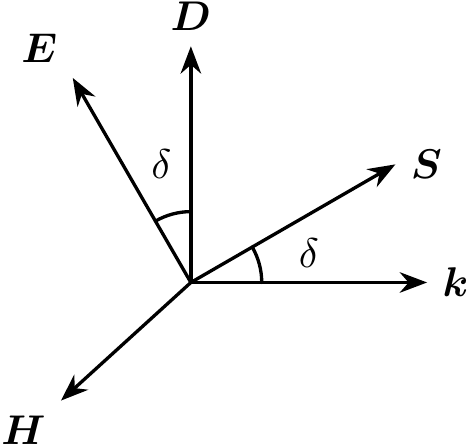
\includegraphics[width=\textwidth]{crystal_optics_fig/electromagnetic_field_vectors_in_crystal.png}
		\caption{晶体内的电磁场矢量}
		\label{晶体内的电磁场矢量}
	\end{minipage}
	\hfill
	\begin{minipage}[b]{0.3\textwidth}
		\centering
		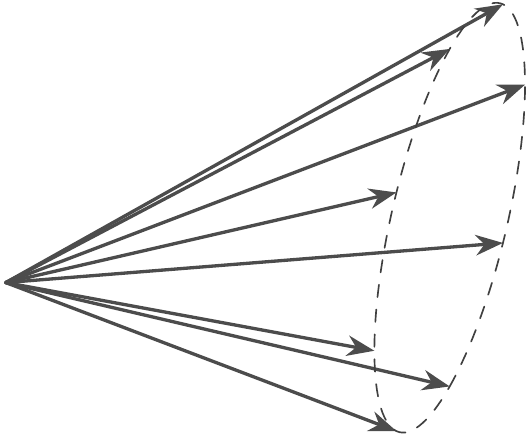
\includegraphics[width=\textwidth]{crystal_optics_fig/conical_refraction_schematic_diagram.png}
		\caption{锥形折射示意图}
		\label{锥形折射示意图}
	\end{minipage}
	\hfill
	\begin{minipage}[b]{0.3\textwidth}
		\centering
		\centering
		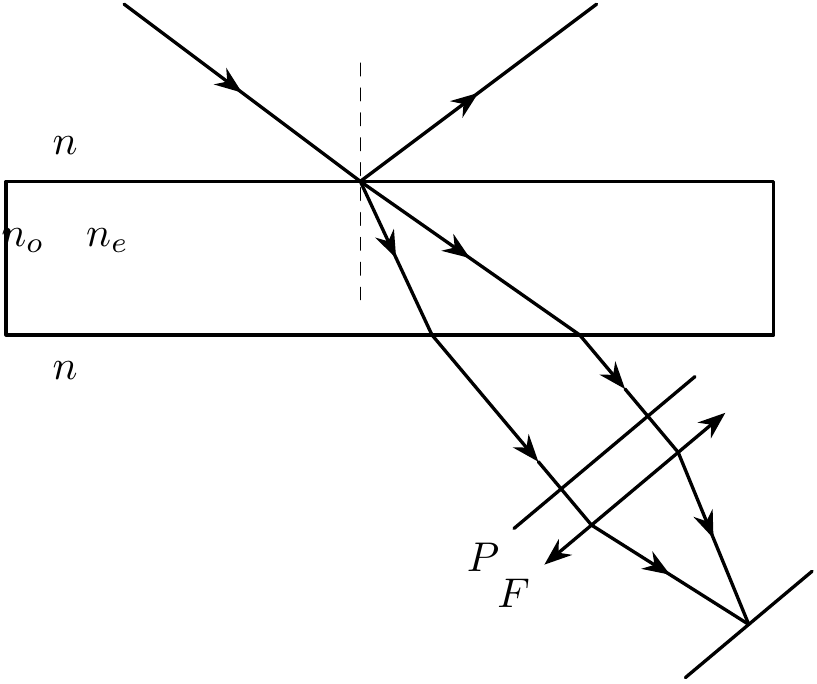
\includegraphics[width=\textwidth]{crystal_optics_fig/interference_setup_schematic_diagram.png}
		\caption{干涉装置示意图}
		\label{干涉装置示意图}
		\label{单轴晶体干涉装置示意图}
	\end{minipage}
\end{figure}

\subsubsection{双轴晶体}
双轴晶体满足\(\varepsilon_1\neq\varepsilon_2\neq\varepsilon_3\)，不妨设\(\varepsilon_1<\varepsilon_2<\varepsilon_3\)，也即\(v_1>v_2>v_3\).

双轴晶体是电各向异性晶体最一般的情形，解析求解极其繁琐，在此仅给出其光轴的定义.

根据相速度方程、群速度方程知，出现重根时
\begin{equation*}
	\tan\xi_r =|\frac{\hat{S}_3}{\hat{S}_1}|=\frac{v_3}{v_1} \sqrt{\frac{v_1^2 - v_2^2}{v_2^2 - v_3^2}},\quad r_2=0,\quad  u'=u''=v_2,
\end{equation*}
\begin{equation*}
	\tan\xi = \tan\xi_N =|\frac{\hat{k}_3}{\hat{k}_1}|= \sqrt{\frac{v_1^2 - v_2^2}{v_2^2 - v_3^2}},\quad n_2=0,\quad  v'=v''=v_2.
\end{equation*}

后者对应的方向定义为光轴，光轴位于最大、最小介电常数对应的主轴所组成的平面内，且与介电常数最大的主轴夹角为\(\pm \xi\).

下特别考虑波矢沿光轴\(+\xi\)传播时的特点，即波矢方向为
\begin{equation*}
	\uv{k} = (\sin\xi, 0, \cos\xi).
\end{equation*}

由于\(\uv{k}\cdot\uv{D}=0\)，不妨设
\begin{equation*}
	\uv{D} = (\sin\varphi \cos\xi, \cos\varphi, -\sin\varphi \sin\xi).
\end{equation*}

进而
\begin{equation*}
	\uv{E} = \frac{\left( \sin\varphi \, v_1^2 \sqrt{v_2^2 - v_3^2}, \, \cos\varphi \, v_2^2 \sqrt{v_1^2 - v_3^2}, \, -\sin\varphi \, v_3^2 \sqrt{v_1^2 - v_2^2} \right)}{\sqrt{v_1^2 - v_3^2} \sqrt{v_2^4 + (v_1^2 - v_2^2)(v_2^2 - v_3^2) \sin^2\varphi}}.
\end{equation*}
\begin{equation*}
	\uv{H} =\uv{k}\times\uv{D}= (-\cos\varphi \cos\xi, \sin\varphi, \cos\varphi \sin\xi).
\end{equation*}
\begin{equation*}
	\uv{S} = \uv{E} \times \uv{H} = \left( \sin\xi \cos\delta - \cos\xi \sin\delta \sin\varphi, \, -\sin\delta \cos\varphi, \, \cos\xi \cos\delta + \sin\xi \sin\delta \sin\varphi \right).
\end{equation*}

其中
\begin{equation*}
	\delta = \angle\left( \uv{E}, \, \uv{D} \right) = \angle\left( \uv{S} \cdot \uv{k} \right) = \arctan\left( \frac{\sqrt{(v_1^2 - v_2^2)(v_2^2 - v_3^2)}}{v_2^2 } |\sin\varphi|\right).
\end{equation*}

可见，若入射自然光，则边界条件的解将取遍\(\varphi\in[\,-\pi/2,\,\pi/2\,]\)，晶体内任意时刻折射光能量所至之点组成细圆环，每一时刻的细圆环组成一个特殊锥面，细圆环便是该特殊锥面垂直于光轴的切面边界.其中，光轴（对应\(\varphi=0\)）与光轴对径处（对应\(\varphi=\pm\pi/2\)）的锥面母线的夹角为
\begin{equation*}
	\psi=\arctan\frac{\sqrt{(v_1^2 - v_2^2)(v_2^2 - v_3^2)}}{v_2^2 }.
\end{equation*}

若入射严格的线偏振光，则根据对称性，边界条件将给出\(\varphi\)与\(\varphi+\pi\)两种模式解，即折射光分为两束.同理，入射椭圆偏振将分出四束折射光，入射更为复杂的偏振组合（但并非各方向均有偏振的自然光）将给出更多束折射光.


\subsubsection{单轴晶体}

单轴晶体中，\(\varepsilon_1=\varepsilon_2,\, v_1=v_2\).

当波矢方向沿3轴，能流方向也沿3轴，偏振矢量在垂直于3轴平面内的任意方向，任意模式的相速度、群速度均为\(v_3\)，此时折射光必定只有一束，故定义3轴为光轴（也可以通过对双轴晶体光轴的表达式取极限得到）.

考虑波矢方向为
\begin{equation*}
	\uv{k} = (\sin\theta \cos\phi, \sin\theta \sin\phi, \cos\theta)
\end{equation*}
的电磁波，取 \(v_2^2 = v_1^2 (1 + \delta)\)，\(|\delta| \ll 1\)，代入波矢方程及 \(E\) 的分量的比例式（通过\(\delta\)取极限）得：
\begin{equation*}
	v' = v_1 \left(1 + \frac{1}{2} \delta \cos^2\phi\right) = v_1, \quad v'' = \sqrt{v_1^2 \cos^2\theta + v_3^2 \sin^2\theta} = v_1 v_3 \sqrt{\frac{v_3^2 \cos^2\xi + v_1^2 \sin^2\xi}{v_3^4 \cos^2\xi + v_1^4 \sin^2\xi}}.
\end{equation*}
\begin{equation*}
	\uv{E}' = (-\sin\phi, \cos\phi, 0), \quad \uv{E}'' = (\cos\xi \cos\phi, \cos\xi \sin\phi, -\sin\xi).
\end{equation*}
其中
\begin{equation*}
	\tan\xi = \frac{v_3^2}{v_1^2} \tan\theta.
\end{equation*}
进而，\(\uv{H}=\uv{k} \times \uv{D}\)可得为
\begin{equation*}
	\uv{H}' = (-\cos\theta \cos\phi, -\cos\theta \sin\phi, \sin\theta), \quad
	\uv{H}'' = (-\sin\phi, \cos\phi, 0)
\end{equation*}
故能流方向\(\uv{S}=\uv{E} \times \uv{H}\) 为
\begin{equation*}
	\uv{S}' = (\sin\theta \cos\phi, \sin\theta \sin\phi, \cos\theta), \quad \uv{S}'' = (\sin\xi \cos\phi, \sin\xi \sin\phi, \cos\xi).
\end{equation*}
进一步按照电磁场本构关系计算得到
\begin{equation*}
	u' = v_1, \quad u'' = \sqrt{\frac{v_1^4 \cos^2\theta + v_3^4 \sin^2\theta}{v_1^2 \cos^2\theta + v_3^2 \sin^2\theta}} = \frac{v_1 v_3}{\sqrt{v_1^2 \sin^2\xi + v_3^2 \cos^2\xi}}.
\end{equation*}

同理，对能流方向为
\begin{equation*}
	\uv{S} = (\sin\xi \cos\phi, \sin\xi \sin\phi, \cos\xi)
\end{equation*}
的电磁波，取 \(v_2^2 = v_1^2\) 的极限得：
\begin{equation*}
	u' = v_1, \quad u'' = \frac{v_1 v_3}{\sqrt{v_1^2 \sin^2\xi + v_3^2 \cos^2\xi}}.
\end{equation*}
\begin{equation*}
	\uv{E}' = (-\sin\phi, \cos\phi, 0), \quad \uv{E}'' = (\cos\xi \cos\phi, \cos\xi \sin\phi, -\sin\xi).
\end{equation*}
进而，\(\uv{H}=\uv{S} \times \uv{E}\)可得为
\begin{equation*}
	\uv{H}' = (-\cos\theta \cos\phi, -\cos\theta \sin\phi, \sin\theta), \quad
	\uv{H}'' = (-\sin\phi, \cos\phi, 0)
\end{equation*}
其中
\begin{equation*}
	\tan\theta = \frac{v_1^2}{v_3^2} \tan\xi.
\end{equation*}
故波矢方向\(\uv{k}=\uv{D} \times \uv{H}\) 为
\begin{equation*}
	\uv{k}' = (\sin\xi \cos\phi, \sin\xi \sin\phi, \cos\xi),
	\quad
	\uv{k}'' = (\sin\theta \cos\phi, \sin\theta \sin\phi, \cos\theta).
\end{equation*}
进一步按照电磁场本构关系计算得到
\begin{equation*}
	v' = v_1, \quad v'' = v_1 v_3 \sqrt{\frac{v_3^2 \cos^2\xi + v_1^2 \sin^2\xi}{v_3^4 \cos^2\xi + v_1^4 \sin^2\xi}} = \sqrt{v_1^2 \cos^2\theta + v_3^2 \sin^2\theta}.
\end{equation*}

通常称 \((v', u')\) 对应寻常模式 (下标o)，\((v'', u'')\) 对应非寻常模式 (下标e)；

将以上结论采用矢量写法，记光轴方向为 \(\uv{x}_3\)，则两类波的波矢、能流密度为
\begin{equation*}
	\vb{k}_o &= \frac{\omega}{v_1} \uv{k}_o, \quad \vb{S}_o = v_1 \uv{k}_o \left(\vb{D}_o \cdot \vb{E}_o\right)\\
	\vb{k}_e &= \frac{\omega}{\sqrt{v_3^2 + (v_1^2 - v_3^2) \left(\uv{k}_e \cdot \uv{x}_3\right)^2}} \uv{k}_e,\quad
	\vb{S}_e = \frac{v_3^2 \uv{k}_e + (v_1^2 - v_3^2) \left(\uv{k}_e \cdot \uv{x}_3\right) \uv{x}_3}{\sqrt{v_3^2 + (v_1^2 - v_3^2) \left(\uv{k}_e \cdot \uv{x}_3\right)^2}} \left(\vb{D}_e \cdot \vb{E}_e\right).
\end{equation*}

电磁场偏振方向为
\begin{equation*}
	\uv{E}_o &= \frac{\uv{x}_3 \times \uv{k}_o}{\left| \uv{x}_3 \times \uv{k}_o \right|}, \quad \uv{H}_o = \frac{\uv{x}_3 - \uv{k}_o \left(\uv{k}_o \cdot \uv{x}_3\right)}{\left| \uv{x}_3 \times \uv{k}_o \right|}\\
	\uv{E}_e &= \frac{\left(\uv{x}_3 \cdot \uv{k}_e\right) v_1^2 \uv{k}_e - \left(v_3^2 + (v_1^2 - v_3^2) \left(\uv{x}_3 \cdot \uv{k}_e\right)^2\right) \uv{x}_3}{\left| \uv{x}_3 \times \uv{k}_e \right| \sqrt{v_3^4 + (v_1^4 - v_3^4) \left(\uv{x}_3 \cdot \uv{k}_e\right)^2}},\quad
	\uv{H}_e = \frac{\uv{x}_3 \times \uv{k}_o}{\left| \uv{x}_3 \times \uv{k}_o \right|}.
\end{equation*}

注意，以上两种情形虽然使用了同一套符号 \((\theta, \xi, \phi)\)，但前者是给定波矢方向求解波的模式，后者是给定能流方向求解波的模式，在物理逻辑和数学技巧上不尽相同.

在大多数单轴晶体中，\(\mu = \mu_0\)，\(\varepsilon_1 = \varepsilon_2 = \varepsilon_0 n_o^2\)，\(\varepsilon_3 = \varepsilon_0 n_e^2\)，上标\('\)的波传播特性与在各向同性介质\(n_o\)传播无异，称为o光，而上标\(''\)的波传播特性较为复杂，需要结合波矢大小、偏振方向和波矢方向的函数关系，根据边界条件具体求解，称为e光.

对于\((\theta, \xi, \phi)\) 方位的e光，其波矢折射率\(n_N\)和能流折射率\(n_r\)记为
\begin{equation*}
	n_N = \frac{c}{v} = \frac{kc}{\omega} = \frac{n_o n_e}{\sqrt{n_o^2 \sin^2\theta + n_e^2 \cos^2\theta}} = \sqrt{\frac{n_o^4 \cos^2\xi + n_e^4 \sin^2\xi}{n_o^2 \cos^2\xi + n_e^2 \sin^2\xi}},
\end{equation*}
\begin{equation*}
	n_r = \frac{c}{u} = \sqrt{n_o^2 \cos^2\xi + n_e^2 \sin^2\xi} = n_e n_o \sqrt{\frac{n_e^2 \cos^2\theta + n_o^2 \sin^2\theta}{n_e^4 \cos^2\theta + n_o^4 \sin^2\theta}},\quad \tan\xi = \frac{n_o^2}{n_e^2} \tan\theta..
\end{equation*}

下考虑一例：

一束角频率为 \(\omega\)的电磁波，一个各向同性介质，折射率为 \(n\).一个单轴晶体，特征折射率为 \(n_o\)，\(n_e\).考虑在两个介质中向左或向右传播的、切向波数为 \(n\omega\sin i/c\) 的四类光.由于寻常光可视为在折射率为 \(n_o\) 的各向同性介质中传播的普通光线，其电场矢量平行于入射面，相关结论称为菲涅尔关系，以下不再赘述，只考虑四类光的非寻常光部分.

假设光轴平行于光线与法线组成的平面，且与法线夹角为 \(\xi\).在透射率和反射率的标记上，切向波矢向右、左以下标\(R\)、\(L\)区分，从晶体打入均匀介质上标\('\)，从均匀介质打入晶体不加上标.

\textbf{先考虑切向波矢向右、从均匀介质打入晶体的光（对应入射角为 \(i\)）.}
\begin{figure}[H]
	\centering
	\begin{subfigure}[b]{0.24\textwidth}
		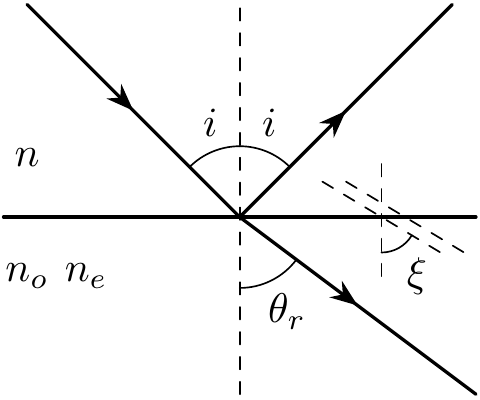
\includegraphics[width=\textwidth]{crystal_optics_fig/birefringent_refraction_case_1.png}
	\end{subfigure}
	\hfill
	\begin{subfigure}[b]{0.24\textwidth}
		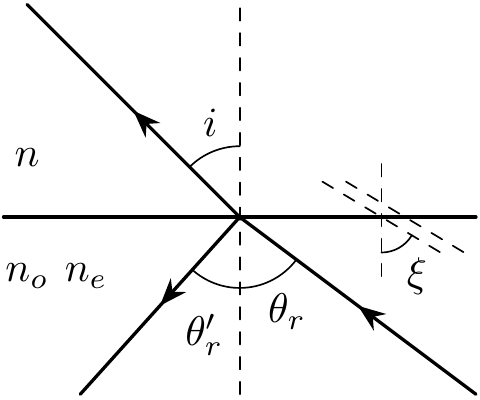
\includegraphics[width=\textwidth]{crystal_optics_fig/birefringent_refraction_case_2.png}
	\end{subfigure}
	\hfill
	\begin{subfigure}[b]{0.25\textwidth}
		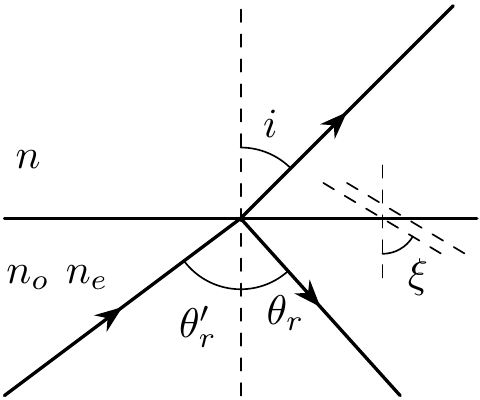
\includegraphics[width=\textwidth]{crystal_optics_fig/birefringent_refraction_case_3.png}
	\end{subfigure}
	\hfill
	\begin{subfigure}[b]{0.25\textwidth}
		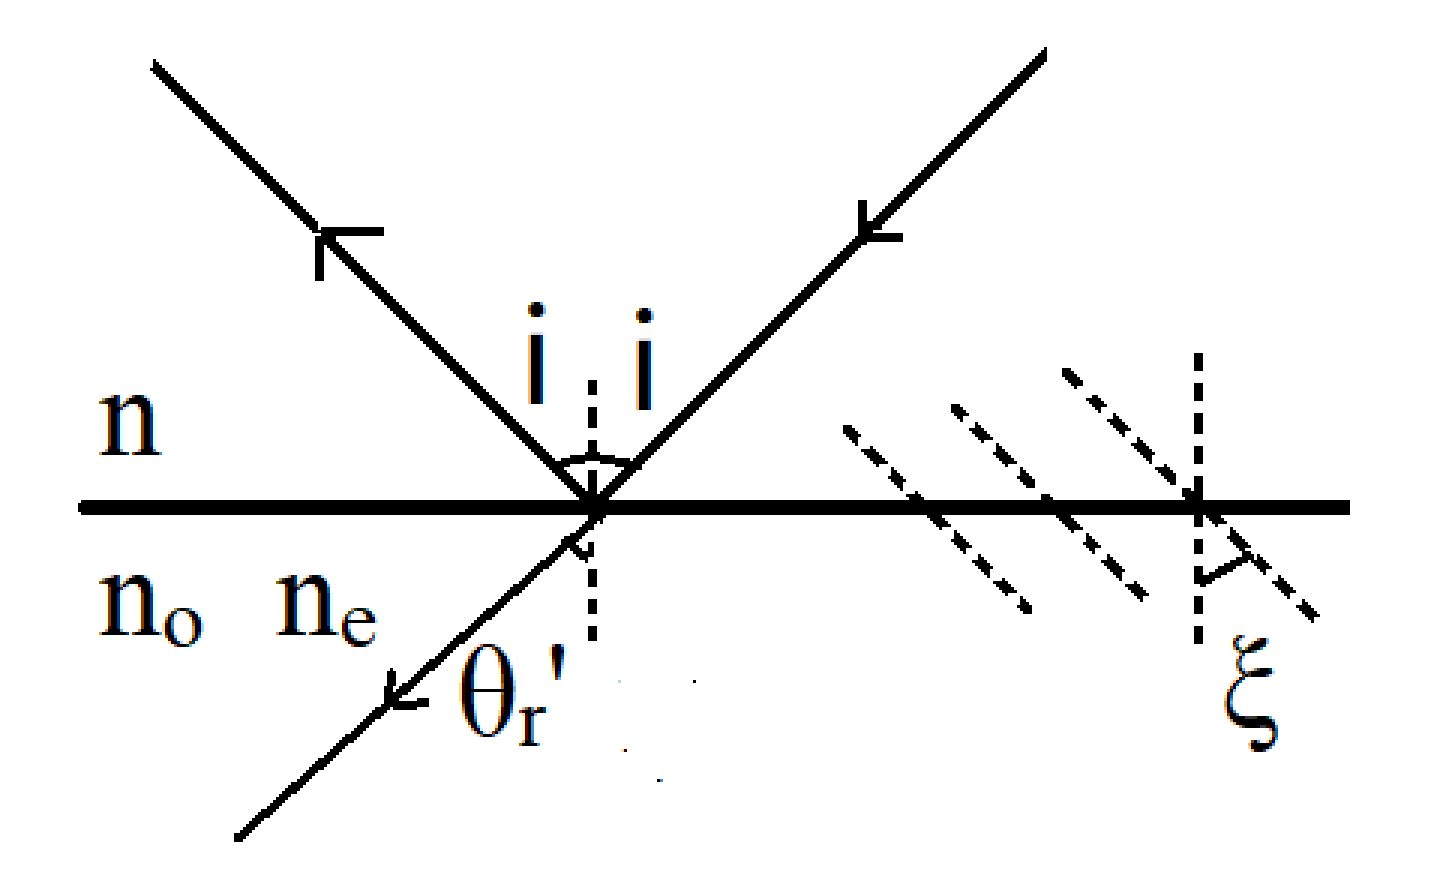
\includegraphics[width=\textwidth]{crystal_optics_fig/birefringent_refraction_case_4.png}
	\end{subfigure}
	\caption{算例的四种出射入射方式}
	\label{算例的四种出射入射方式}
\end{figure}

记透射光线与法线的夹角 \(\theta_r\)、透射光波矢与法线夹角 \(\theta_N\).根据如上所求，\(\theta_N\) 方向的折射率为：
\begin{equation*}
	n_N = \dfrac{n_o n_e}{\sqrt{n_e^2 \cos^2(\theta_N - \xi) + n_o^2 \sin^2(\theta_N - \xi)}}.
\end{equation*}

由折射定律 \(n \sin i = n_N \sin \theta_N\)，解得：
\begin{equation*}
	\theta_N = \xi + \arctan\left( \dfrac{n_e \left( n_o n_e \sin\xi \cos\xi - n \sin i \sqrt{n_e^2 \cos^2\xi + n_o^2 \sin^2\xi - n^2 \sin^2 i} \right)}{n_o \left( n^2 \sin^2 i - n_e^2 \cos^2\xi \right)} \right).
\end{equation*}

因此：
\begin{equation*}
	\theta_r = \xi + \arctan\left( \dfrac{n_o^2}{n_e^2} \tan(\theta_N - \xi) \right) = \xi + \arctan\left( \dfrac{n_o \left( n_o n_e \sin\xi \cos\xi - n \sin i \sqrt{n_e^2 \cos^2\xi + n_o^2 \sin^2\xi - n^2 \sin^2 i} \right)}{n_e \left( n^2 \sin^2 i - n_e^2 \cos^2\xi \right)} \right).
\end{equation*}

电磁场方程给出：
\begin{equation*}
	\vb{H} = \sqrt{\dfrac{\varepsilon_0}{\mu_0}} n_N \uv{k} \times \vb{E}, \quad \vb{S} = \vb{E} \times \vb{H} = \sqrt{\dfrac{\varepsilon_0}{\mu_0}} n_N \vb{E} \times (\uv{k} \times \vb{E}).
\end{equation*}

故 \(\vb{E}\)，\(\vb{H}\) 切向分量连续可写作：
\begin{equation*}
	(E_i - E_r) \cos i = E_t \cos\theta_r, \quad n (E_i + E_r) = n_N E_t \cos(\theta_r - \theta_N).
\end{equation*}

解得电场矢量的反射率为：
\begin{equation*}
	r_R = \dfrac{E_r}{E_i} = \dfrac{n_o n_e \cos i - n \sqrt{n_e^2 \cos^2\xi + n_o^2 \sin^2\xi - n^2 \sin^2 i}}{n_o n_e \cos i + n \sqrt{n_e^2 \cos^2\xi + n_o^2 \sin^2\xi - n^2 \sin^2 i}}.
\end{equation*}

电场矢量的透射率为：
\begin{equation*}
	t_R = \dfrac{E_t}{E_i} = \dfrac{2 n \cos i \sqrt{n_e^2 \cos^2\xi + n_o^2 \sin^2\xi - n^2 \sin^2 i}}{\cos\theta_r \left( n_o n_e \cos i + n \sqrt{n_e^2 \cos^2\xi + n_o^2 \sin^2\xi - n^2 \sin^2 i} \right)}.
\end{equation*}

进而能流密度反射率为：
\begin{equation*}
	R_R = r_p^2 = \left( \dfrac{n_o n_e \cos i - n \sqrt{n_e^2 \cos^2\xi + n_o^2 \sin^2\xi - n^2 \sin^2 i}}{n_o n_e \cos i + n \sqrt{n_e^2 \cos^2\xi + n_o^2 \sin^2\xi - n^2 \sin^2 i}} \right)^2.
\end{equation*}

能流密度透射率为：
\begin{equation*}
	T_R = \dfrac{1}{n} n_N \cos(\theta_r - \theta_N) \,t_R^2 = \dfrac{4 n_o n_e n \cos^2 i \sqrt{n_e^2 \cos^2\xi + n_o^2 \sin^2\xi - n^2 \sin^2 i}}{\cos\theta_r \left( n \sqrt{n_e^2 \cos^2\xi + n_o^2 \sin^2\xi - n^2 \sin^2 i} + n_o n_e \cos i \right)^2}.
\end{equation*}

易证，以上所求满足能量守恒关系：
\begin{equation*}
	R_R + T_R \dfrac{\cos\theta_r}{\cos i} = 1.
\end{equation*}

\textbf{再考虑切向波矢向左、从晶体打入均匀介质的光，显然，其出射角为 \(i\).}

记入射光线与法线的夹角 \(\theta_r'\)、波矢与法线夹角 \(\theta_N'\).\(\theta_N'\) 方向折射率为：
\begin{equation*}
	n_N' = \dfrac{n_o n_e}{\sqrt{n_e^2 \cos^2(\theta_N' + \xi) + n_o^2 \sin^2(\theta_N' + \xi)}}.
\end{equation*}

由折射定律 \(n \sin i = n_N' \sin \theta_N'\)，解得：
\begin{equation*}
	\theta_N' = -\xi - \arctan\left( \dfrac{n_e \left( n_o n_e \sin\xi \cos\xi + n \sin i \sqrt{n_e^2 \cos^2\xi + n_o^2 \sin^2\xi - n^2 \sin^2 i} \right)}{n_o \left( n^2 \sin^2 i - n_e^2 \cos^2\xi \right)} \right).
\end{equation*}

因此：
\begin{equation*}
	\theta_r' = -\xi + \arctan\left( \dfrac{n_o^2}{n_e^2} \tan(\theta_N' + \xi) \right) = -\xi - \arctan\left( \dfrac{n_o \left( n_o n_e \sin\xi \cos\xi + n \sin i \sqrt{n_e^2 \cos^2\xi + n_o^2 \sin^2\xi - n^2 \sin^2 i} \right)}{n_e \left( n^2 \sin^2 i - n_e^2 \cos^2\xi \right)} \right).
\end{equation*}

由 \(\vb{E}\)，\(\vb{H}\) 切向分量连续：
\begin{equation*}
	E_i' \cos\theta_r - E_r' \cos\theta_r' = E_t' \cos i,\quad
	n_N \cos(\theta_r - \theta_N) E_i' + n_N' \cos(\theta_r' - \theta_N') E_r' = n E_t'.
\end{equation*}

解得：
\begin{align*}
	r_L' & = \dfrac{E_r'}{E_i'} = -\dfrac{ n_o n_e \cos i - n \sqrt{n_e^2 \cos^2\xi + n_o^2 \sin^2\xi - n^2 \sin^2 i} }{ n_o n_e \cos i + n \sqrt{n_e^2 \cos^2\xi + n_o^2 \sin^2\xi - n^2 \sin^2 i} } \cdot \dfrac{\cos\theta_r}{\cos\theta_r'}, \\
	t_L' & = \dfrac{E_t'}{E_i'} = \dfrac{2 n_o n_e \cos\theta_r}{n_o n_e \cos i + n \sqrt{n_e^2 \cos^2\xi + n_o^2 \sin^2\xi - n^2 \sin^2 i}}.
\end{align*}

进而：
\begin{align*}
	R_L' & = \dfrac{(r_L')^2 n_N' \cos(\theta_r' - \theta_N')}{n_N \cos(\theta_r - \theta_N)} = \left( \dfrac{n_o n_e \cos i - n \sqrt{n_e^2 \cos^2\xi + n_o^2 \sin^2\xi - n^2 \sin^2 i}}{n_o n_e \cos i + n \sqrt{n_e^2 \cos^2\xi + n_o^2 \sin^2\xi - n^2 \sin^2 i}} \right)^2 \cdot \dfrac{\cos\theta_r}{\cos\theta_r'}, \\
	T_L' & = \dfrac{n (t_L')^2}{n_N \cos(\theta_r - \theta_N)} = \dfrac{4 n_o n_e n \sqrt{n_e^2 \cos^2\xi + n_o^2 \sin^2\xi - n^2 \sin^2 i} \cos\theta_r}{\left( n \sqrt{n_e^2 \cos^2\xi + n_o^2 \sin^2\xi - n^2 \sin^2 i} + n_o n_e \cos i \right)^2}.
\end{align*}

易证，以上所求满足能量守恒关系：
\begin{equation*}
	\dfrac{\cos i}{\cos\theta_r} T_L' + \dfrac{\cos\theta_r'}{\cos\theta_r} R_L' = 1.
\end{equation*}

计算中用到关系式
\begin{equation*}
	\dfrac{\cos\theta_r \sin\theta_N}{\cos(\theta_r - \theta_N)} = \dfrac{\cos\theta_r' \sin\theta_N'}{\cos(\theta_r' - \theta_N')} = \dfrac{n \sin i}{n_o n_e} \sqrt{n_e^2 \cos^2\xi + n_o^2 \sin^2\xi - n^2 \sin^2 i}.
\end{equation*}

\textbf{
	在求得以上两种情形后，根据斯托克斯关系，对于所有切向波矢为 \(\pm n\omega\sin i/c\) 的出射入射组合，其反射率和透射率都可快速求出.}

\begin{figure}[H]
	\centering
	\begin{subfigure}[b]{0.33\textwidth}
		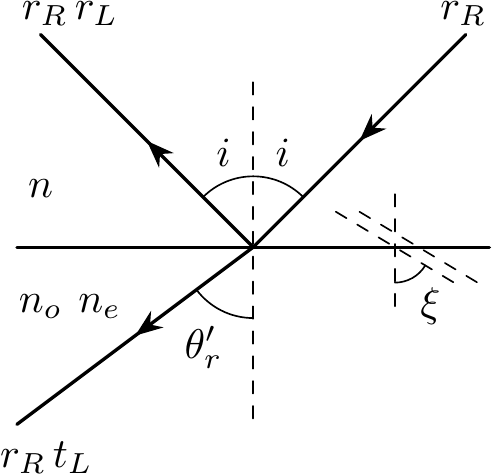
\includegraphics[width=\textwidth]{crystal_optics_fig/first_extinction_case_left_panel.png}
	\end{subfigure}
	\hfill
	\begin{subfigure}[b]{0.32\textwidth}
		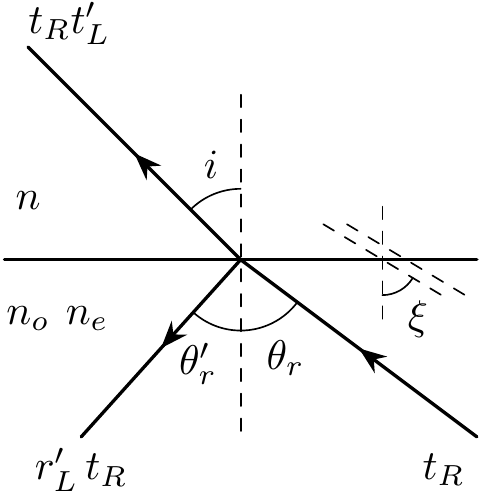
\includegraphics[width=\textwidth]{crystal_optics_fig/first_extinction_case_middle_panel.png}
	\end{subfigure}
	\hfill
	\begin{subfigure}[b]{0.33\textwidth}
		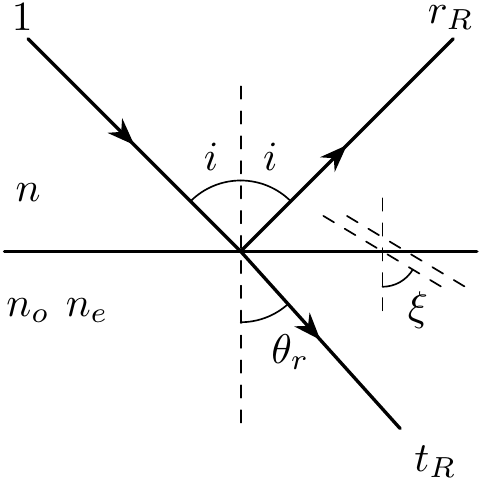
\includegraphics[width=\textwidth]{crystal_optics_fig/first_extinction_case_right_panel.png}
	\end{subfigure}
	\caption{第一类消光情形}
	\label{第一类消光情形}
\end{figure}

如图\ref{第一类消光情形}，该情形可消光，则：
\begin{equation*}
	r_R r_L + t_R t_L' = 1, \quad r_R t_L + r_L' t_R = 0.
\end{equation*}
\begin{figure}[H]
	\centering
	\begin{subfigure}[b]{0.33\textwidth}
		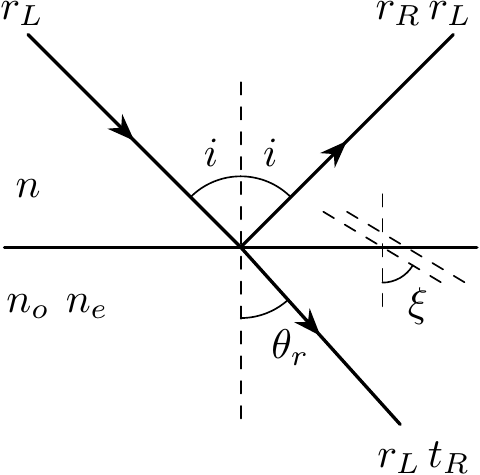
\includegraphics[width=\textwidth]{crystal_optics_fig/second_extinction_case_left_panel.png}
	\end{subfigure}
	\hfill
	\begin{subfigure}[b]{0.32\textwidth}
		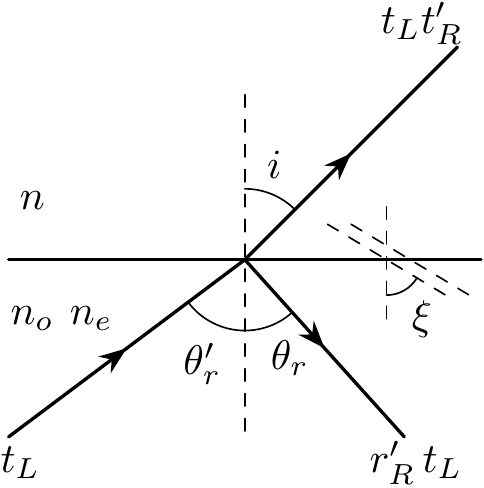
\includegraphics[width=\textwidth]{crystal_optics_fig/second_extinction_case_middle_panel.png}
	\end{subfigure}
	\hfill
	\begin{subfigure}[b]{0.33\textwidth}
		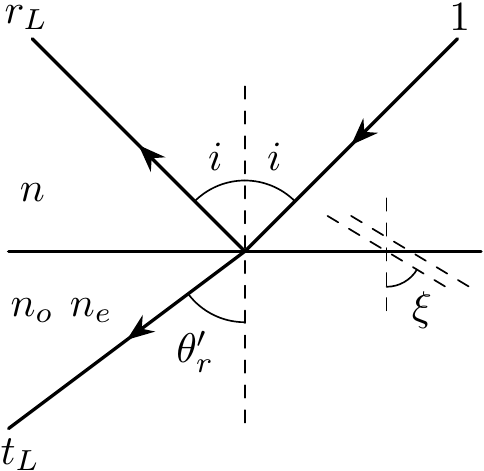
\includegraphics[width=\textwidth]{crystal_optics_fig/second_extinction_case_right_panel.png}
	\end{subfigure}
	\caption{第二类消光情形}
	\label{第二类消光情形}
\end{figure}

如图\ref{第二类消光情形}，该情形可消光，则：
\begin{equation*}
	r_R r_L + t_L t_R' = 1, \quad r_L t_R + r_R' t_L = 0.
\end{equation*}
解得：
\begin{equation*}
	t_L' = \dfrac{1 - r_R r_L}{t_R}, \quad r_L' = -\dfrac{r_R t_L}{t_R}, \quad t_R' = \dfrac{t_R}{t_L} t_L', \quad r_R' = \dfrac{r_R r_L}{r_L'}.
\end{equation*}
这说明 \(r_R, t_R, r_L, t_L, r_R', t_R', r_L', t_L'\) 共8个振幅反射透射率中，只有4个是独立的.

另由能量守恒，易得：
\begin{equation*}
	\begin{pmatrix}
		-1   & R_R  & T_R  & 0    \\
		R_L  & -1   & 0    & T_L  \\
		T_L' & 0    & -1   & R_L' \\
		0    & T_R' & R_R' & -1
	\end{pmatrix}
	\begin{pmatrix}
		\cos i       \\
		\cos i       \\
		\cos\theta_r \\
		\cos\theta_r'
	\end{pmatrix} = 0.
\end{equation*}
在求出各角度参量后，也可根据该关系推出各能量反射透射率.比如，若给定 \(n, i, n_o, n_e, \xi\)，则只需求出 \(\theta_r\)、\(\theta_r'\)、\(r_R\)、\(t_R\)，根据斯托克斯关系，便可以快速求出共16个振幅、能量的反射透射率.

注意到，对于替换\(i \to -i\)，\(r_R\) 不变，\(t_R \cos\theta_r\) 不变，因此：
\begin{equation*}
	r_L = r_R, \quad t_L = \dfrac{\cos\theta_r}{\cos\theta_r'} t_R.
\end{equation*}

易知，\(R_R = r_R^2\)，\(R_L = r_R^2\)，则：
\begin{equation*}
	T_R = \dfrac{(1 - r_R^2) \cos i}{\cos\theta_r}, \quad T_L = \dfrac{(1 - r_R^2) \cos i}{\cos\theta_r'}.
\end{equation*}

注意到 \(R_L' = r_R^2 \dfrac{\cos\theta_r}{\cos\theta_r'}\)，故 \begin{equation*}
	R_R' = \dfrac{\cos\theta_r'}{\cos\theta_r} r_R^2,\quad T_R' = (1 - r_R^2) \dfrac{\cos\theta_r'}{\cos i},\quad T_L' = (1 - r_R^2) \dfrac{\cos\theta_r}{\cos i}
\end{equation*}

另由斯托克斯关系式得：
\begin{equation*}
	r_L' = -r_R \dfrac{\cos\theta_r}{\cos\theta_r'}, \quad t_L' = \dfrac{1 - r_R^2}{t_R},
\end{equation*}
\begin{equation*}
	r_R' = -r_R \dfrac{\cos\theta_r'}{\cos\theta_r}, \quad t_R' = \dfrac{1 - r_R^2}{t_R} \cdot \dfrac{\cos\theta_r'}{\cos\theta_r}.
\end{equation*}


比如，对于具体数据 \((n = 1, i = 7^\circ, \xi = 17^\circ, n_o = 1.4, n_e = 1.6)\)，计算得：
\begin{equation*}
	&\theta_r = 0.13495 \, \text{rad}, \quad \theta_N = 0.086714 \, \text{rad}, \quad \theta_r' = 0.0020357 \, \text{rad}, \quad \theta_N' = 0.085722 \, \text{rad}.\\
	&r_R = 0.16939, \quad R_R = 0.028693, \quad t_R = 0.83198, \quad T_R = 0.97291.\\
	&r_L' = -0.16785, \quad R_L' = 0.028432, \quad t_L' = 1.1675, \quad T_L' = 0.96970.\\
	&r_L = 0.16939, \quad R_L = 0.028693, \quad t_L = 0.82442, \quad T_L = 0.96407.\\
	&r_R' = -0.17094, \quad R_R' = 0.028956, \quad t_R' = 1.1782, \quad T_R' = 0.97860.
\end{equation*}

如果从均匀介质向右打光至长方体单轴晶体，晶体厚度为\(h\)，则在出射晶体后，o光和e光平行但不重合，其相位差为：
\begin{align*}
	\Delta\phi & = \dfrac{\omega}{c} h \left( n_N \cos\theta_N - n_o \cos\theta_0 \right)                                                                                                                                                                                                  \\
	           & =\dfrac{\omega h}{c} \left( \frac{n_o \left( n^2 \sin^2 i - n_e^2 \right) + n n_e \sin i \tan\xi \sqrt{n_e^2 \cos^2\xi + n_o^2 \sin^2\xi - n^2 \sin^2 i}}{n n_o \sin i \tan\xi - n_e \sqrt{n_e^2 \cos^2\xi + n_o^2 \sin^2\xi - n^2 \sin^2 i}} - n_o \cos\theta_0 \right).
\end{align*}

进而可通过偏振片、凸透镜使之同方向并汇聚干涉（如图\ref{单轴晶体干涉装置示意图}）.

各项同性晶体受外界因素扰动可能变成单轴晶体，其两个特征折射率相差不大，\(n_e = n_o(1 + \delta)\)，\(|\delta| \ll 1\)，可近似得
\begin{align*}
	\theta_N   & = \theta_o - \tan\theta_o \sin^2(\theta_o - \xi) \delta,
	\theta_N' = \theta_o - \tan\theta_o \sin^2(\theta_o + \xi) \delta,                                     \\
	\theta_r   & = \theta_o - \tan\theta_o \sin^2(\theta_o - \xi) \delta - \sin(2(\theta_o - \xi)) \delta,
	\theta_r' = \theta_o - \tan\theta_o \sin^2(\theta_o + \xi) \delta - \sin(2(\theta_o + \xi)) \delta,    \\
	n_N        & = \dfrac{n \sin i}{\sin\theta_o} \left( 1 + \sin^2(\theta_o - \xi) \delta \right),
	n_N' = \dfrac{n \sin i}{\sin\theta_o} \left( 1 + \sin^2(\theta_o + \xi) \delta \right),                \\
	\Delta\phi & = \dfrac{\omega}{c} n_o h \cdot \dfrac{\sin^2(\theta_o - \xi)}{\cos\theta_o} \delta
\end{align*}

注意到，\(\Delta\phi\propto\,\delta\)，进而可以通过干涉条纹间距的变化来测量所施加的外部扰动.

特别地，若 \(\xi = 0\)，则：
\begin{equation*}
	\theta_N' &= \theta_N = \arctan\left( \dfrac{n_e n \sin i}{n_o \sqrt{n_e^2 - n^2 \sin^2 i}} \right),
	\theta_r' = \theta_r = \arctan\left( \dfrac{n_o n \sin i}{n_e \sqrt{n_e^2 - n^2 \sin^2 i}} \right),\\
	r_R &= r_L = -r_R' = -r_L' = \dfrac{n_o n_e \cos i - n \sqrt{n_e^2 - n^2 \sin^2 i}}{n_o n_e \cos i + n \sqrt{n_e^2 - n^2 \sin^2 i}},\\
	t_R &= t_L = \dfrac{2 n \cos i \sqrt{n_e^4 + (n_o^2 - n_e^2) n^2 \sin^2 i}}{n_e \left( n_o n_e \cos i + n \sqrt{n_e^2 \cos^2\xi + n_o^2 \sin^2\xi - n^2 \sin^2 i} \right)},\\
	t_R' &= t_L' = \dfrac{2 n_o n_e^2 \sqrt{n_e^2 - n^2 \sin^2 i}}{\sqrt{n_e^4 + (n_o^2 - n_e^2) n^2 \sin^2 i} \left( n_o n_e \cos i + n \sqrt{n_e^2 \cos^2\xi + n_o^2 \sin^2\xi - n^2 \sin^2 i} \right)},\\
	R_R &= R_L = R_R' = R_L' = \left( \dfrac{n_o n_e \cos i - n \sqrt{n_e^2 - n^2 \sin^2 i}}{n_o n_e \cos i + n \sqrt{n_e^2 - n^2 \sin^2 i}} \right)^2,\\
	T_R &= T_L = \dfrac{4 n_o n \cos^2 i \sqrt{n_e^4 + (n_o^2 - n_e^2) n^2 \sin^2 i}}{\left( n_o n_e \cos i + n \sqrt{n_e^2 \cos^2\xi + n_o^2 \sin^2\xi - n^2 \sin^2 i} \right)^2},\\
	T_R' &= T_L' = \dfrac{4 n_o n_e^2 n (n_e^2 - n^2 \sin^2 i)}{\sqrt{n_e^4 + (n_o^2 - n_e^2) n^2 \sin^2 i} \left( n \sqrt{n_e^2 \cos^2\xi + n_o^2 \sin^2\xi - n^2 \sin^2 i} + n_o n_e \cos i \right)^2}.
\end{equation*}

特别地，若 \(\xi = \pi/2\)，则：
\begin{equation*}
	\theta_N' &= \theta_N = \arctan\left( \dfrac{n_o n \sin i}{n_e \sqrt{n_o^2 - n^2 \sin^2 i}} \right),
	\theta_r'= \theta_r = \arctan\left( \dfrac{n_e n \sin i}{n_o \sqrt{n_o^2 - n^2 \sin^2 i}} \right),\\
	r_R &= r_L = -r_R' = -r_L' = \dfrac{n_o n_e \cos i - n \sqrt{n_o^2 - n^2 \sin^2 i}}{n_o n_e \cos i + n \sqrt{n_o^2 - n^2 \sin^2 i}},\\
	t_R &= t_L = \dfrac{2 n \cos i \sqrt{n_o^4 + (n_e^2 - n_o^2) n^2 \sin^2 i}}{n_o \left( n_o n_e \cos i + n \sqrt{n_o^2 - n^2 \sin^2 i} \right)},\\
	R_R &= R_L = R_R' = R_L' = \left( \dfrac{n_o n_e \cos i - n \sqrt{n_o^2 - n^2 \sin^2 i}}{n_o n_e \cos i + n \sqrt{n_o^2 - n^2 \sin^2 i}} \right)^2,\\
	T_R &= T_L = \dfrac{4 n_e n \cos^2 i \sqrt{n_o^4 + (n_e^2 - n_o^2) n^2 \sin^2 i}}{\left( n \sqrt{n_e^2 \cos^2\xi + n_o^2 \sin^2\xi - n^2 \sin^2 i} + n_o n_e \cos i \right)^2},\\
	T_R' &= T_L' = \dfrac{4 n_o^2 n_e n (n_o^2 - n^2 \sin^2 i)}{\sqrt{n_o^4 + (n_e^2 - n_o^2) n^2 \sin^2 i} \left( n \sqrt{n_e^2 \cos^2\xi + n_o^2 \sin^2\xi - n^2 \sin^2 i} + n_o n_e \cos i \right)^2}.
\end{equation*}

特别地，若 \(i = 0\)，则：
\begin{equation*}
	\theta_N' &= \theta_N = 0, \quad \theta_r' = -\theta_r = -\xi + \arctan\left( \dfrac{n_o^2}{n_e^2} \tan\xi \right),\\
	r_R &= r_L = -r_R' = -r_L' = \dfrac{n_o n_e - n \sqrt{n_e^2 \cos^2\xi + n_o^2 \sin^2\xi}}{n_o n_e + n \sqrt{n_e^2 \cos^2\xi + n_o^2 \sin^2\xi}},\\
	t_R &= t_L = \dfrac{2 n \sqrt{n_e^2 \cos^2\xi + n_o^2 \sin^2\xi}\,\sqrt{n_e^4 \cos^2\xi + n_o^4 \sin^2\xi}}{\left( n_e^2 \cos^2\xi + n_o^2 \sin^2\xi \right) \left( n_o n_e + n \sqrt{n_e^2 \cos^2\xi + n_o^2 \sin^2\xi} \right)},\\
	t_R' &= t_L' = \dfrac{2 n_o n_e \left( n_e^2 \cos^2\xi + n_o^2 \sin^2\xi \right)}{\sqrt{n_e^4 \cos^2\xi + n_o^4 \sin^2\xi} \left( n_o n_e + n \sqrt{n_e^2 \cos^2\xi + n_o^2 \sin^2\xi} \right)},\\
	R_R &= R_L = R_R' = R_L' = \left( \dfrac{n_o n_e - n \sqrt{n_e^2 \cos^2\xi + n_o^2 \sin^2\xi}}{n_o n_e + n \sqrt{n_e^2 \cos^2\xi + n_o^2 \sin^2\xi}} \right)^2,\\
	T_R &= T_L = \dfrac{4 n_o n_e n \sqrt{n_e^2 \cos^2\xi + n_o^2 \sin^2\xi}\,\sqrt{n_e^4 \cos^2\xi + n_o^4 \sin^2\xi}}{\left( n_e^2 \cos^2\xi + n_o^2 \sin^2\xi \right) \left( n \sqrt{n_e^2 \cos^2\xi + n_o^2 \sin^2\xi} + n_o n_e \right)^2},\\
	T_R' &= T_L' = \dfrac{4 n_o n_e n \sqrt{n_e^2 \cos^2\xi + n_o^2 \sin^2\xi} \left( n_e^2 \cos^2\xi + n_o^2 \sin^2\xi \right)}{\sqrt{n_e^4 \cos^2\xi + n_o^4 \sin^2\xi} \left( n \sqrt{n_e^2 \cos^2\xi + n_o^2 \sin^2\xi} + n_o n_e \right)^2}.
\end{equation*}
